\documentclass{article}
\usepackage{listings}
\usepackage{enumerate}
\usepackage{graphicx}
\graphicspath{{Pictures/}}

\begin{document}
\pagenumbering{gobble}
\title{Homework \#3}
\author{Chris Dellomes\\
Professor: Ray Toal\\
CMSI 282: Algorithms\\
Loyola Marymount University}

\date{April 7, 2015}

\maketitle

\clearpage
\begin{enumerate}
	\item \begin{lstlisting}
from random import randint
def bozosort(list):
    toSort = list
    sorted = False
    runs = 0
    while sorted == False:
        sorted = True
        for i in range(0, len(toSort)-1):
            if toSort[i] > toSort[i+1]:
                sorted = False;
        if sorted == False:
            rand1 = randint(0, len(toSort)-1)
            rand2 = randint(0, len(toSort)-1)
            while rand1 == rand2:
                rand1 = randint(0, len(toSort)-1)
                rand2 = randint(0, len(toSort)-1)
            old_toSort1 = toSort[rand1]
            toSort[rand1] = toSort[rand2]
            toSort[rand2] = old_toSort1
            runs += 1
            print(toSort)
    return toSort
    \end{lstlisting}

    \begin{center}
    \begin{tabular}{c c}
    List Length & Average Number of Steps Over 1000 Trials\\
    2 & 1.0\\
    3 & 6.082\\
    4 & 26.726\\
    5 & 131.11\\
    6 & 771.524
    \end{tabular}
    \end{center}


    \item \begin{lstlisting}
def autokey(plaintext, keyphrase):
    key = list(keyphrase.upper())
    message = list(plaintext.upper())
    for i in range(0, len(message) - len(key)):
        key.append(message[i])
    ciphertext = []
    for j in range(0, len(key)):
        codepoint = ord(key[j]) + ord(message[j]) - 65
        if codepoint > 90:
            codepoint -= 26
        ciphertext.append(chr(codepoint))
    return ''.join(ciphertext)
	\end{lstlisting}

    \clearpage

	\item We implement frequency analysis and guessing to reconstrunct the mapping of letters. We first note the most frequent letters are Q, W, O, R, M and try to correspond them to other letters
    like E, T, A, O, I, that are on average the most frequent in sentences. We also notice N, C, Z, G, Y are not in the ciphertext, which corresponds to infrequent letters like Z, Q, and X. From there, we use patterns and more matchings of frequencies to generate guesses.

    \clearpage

    \begin{lstlisting}
    UIQLDEVORHIWLTQTOKMQMWROUOQQMQLKIQWQVIEWRDQTLEQMWRWXFTWHTOAD
    MRDQIOKWXMAOHMRMRHQVOQWLTAOMRQODPMDQWMRDQTLEQOEWAFLQITBVOQQW
    KWUIQLDEWREIRQTOQITOQVITWRIJFUOMRMRHQWVLAORSIMRHDBVOQBIBORQO
    EWAFLQITQWKW

    UITLDEVANHIOLTTTAKITIONAUATTITLKITOTVIEONDTTLETIONOXFTOHTAAD
    INDTIAKOXIAAHININHTVATOLTAAINTADPIDTOINDTTLETAEOAFLTITBVATTO
    KOUITLDEONEINTTATITATVITONIJFUAININHTOVLAANSIINHDBVATBIBANTA
    EOAFLTITTOKO

    UITLDEVANHIOLTTTAKITIONAUATTITLKITOTVIEONDTTLETIONOXFTOHTAIDI
    NDTIAKOXIIAHININHTVATOLTIAINTADPIDTOINDTTLETAEOIFLTITOVATTOKO
    UITLDEONEINTTATITATVITONIJFUAININHTOVLIANSIINHDOVATOIOANTAEOI
    FLTITTOKO

    LETLDEVANHEOLTTTAKITIONALATTITLKETOTVEEONDTTLETIONOXFTOHTAIDI
    NDTEAKOXIIAHININHTVATOLTIAINTADPIDTOINDTTLETAEOIFLTETOVATTOKO
    LETLDEONEENTTATETATVETONEJFLAININHTOVLIANSEINHDOVATOEOANTAEOI
    FLTETTOKO

    LETLDCVANHEOLTTTADITIONALATTITLDETOTVECONDTTLCTIONOXXTOHTAIDI
    NDTEADOXIIAHININHTVATOLTIAINTADPIDTOINDTTLCTACOIXLTETOVATTODO
    LETLDCONCENTTATETATVETONEJXLAININHTOVLIANSEINHDOVATOEOANTACOI
    XLTETTODO

    LETUSCVANHEOURTRADITIONALATTITUDETOTVECONSTRUCTUINOFFROHRAISI
    NSTEADOXIIAHININHTVATOURIAINTASPISTOINSTRUCTACOIFUTEROVATTODO
    LETUSCONCENTRATERATVERONEJFLAININHTOVUMANSEINHSOVATOEOAMTACOI
    FUTERTODO

    LETUSCHANGEOURTRADITIONALATTITUDETOTHECONSTRUCTIONOFPROGRAMSI
    NSTEADOFIMAGININGTHATOURMAINTASKISTOINSTRUCTACOMPUTERWHATTODO
    LETUSCONCENTRATERATHERONEXPLAININGTOHUMANBEINGSWHATWEWANTACOMP
    UTERTODO
    \end{lstlisting}

    Let us change our traditional attitude to the construction of programs instead of imagining that our main task is to instruct a computer what to do let us concentrate rather on explaining to human beings what we want a computer to do.

	\clearpage

	\item
Polybius Square

d	a	r	n	o

t	h	e	c	y

p	l	s	i	q

u	b	f	g	k

m	v	w	x	z

Mapping

t - 1, 0

w - 4, 2

b - 3, 1

l - 2, 1

a - 0, 1

e - 1, 2

p - 2, 0

o - 0, 4

d - 0, 0

u - 3, 0

v - 4, 1

s - 2, 2

n - 0, 3

h - 1, 1

k - 3, 4

i - 2, 3

f - 3, 2

g - 3, 3

m - 4, 0

y - 1, 4

q - 2, 4

r - 0, 2

Translation

10 42 31 10 21 21 01 12 20 04 00 10 30 31 10 42 31 10 21 10 00 21 00 00 41 22 03 03 11 12 12 10 21 22 | 34 00 00 22 23 32 33 23 23 40 42 21 14 00 34 00 00 22 20 11 31 20 24 34 04 32 11 40 00 21 22 34 02 22
\clearpage
Shift

13 04 40 20 30 10 12 02 22 13 23 12 03 13 12 23 22 03 04 40 04 02 12 01 31 04 30 10 13 04 40 20 30 10 12 02 22 10 11 01 03 01 22 10 02 04 03 04 40 14 23 22 01 31 04 30 10 10 12 21 12 21 12 22 13 04 20 12 22 22

Decipher

c o m p u t e r s c i e n c e i s n o m o r e a b o u t c o m p u t e r s t h a n a s t r o n o m y i s a b o u t t e l e s c o p e s s

computer science is no more about computers than astronomy is about telescopes

	\item First, we factor the N value of the public key to find the p and q values. Then we use the extended euclidean algorithm to find the modular inverse of the e value from
    the public key and the p - 1 and q - 1 values. The result is the private key, which comes out to be 583903097165.
    \clearpage
    \begin{lstlisting}
import math

def extended_euclidean(a, b):
    if a == 0:
        return (b, 0, 1)
    g, y, x = extended_euclidean(b % a, a)
    return g, x - math.floor(b / a) * y, y

def modular_inverse(a, mod):
    g, x, y = extended_euclidean(a, mod)
    if g != 1:
        return False
    return x % mod

def is_square(n):
    if math.sqrt(n) == int(math.sqrt(n)):
        return True
    return False

def factor(n):
    a = math.ceil(math.sqrt(n))
    b = (a ** 2) - n
    while is_square(b) == False:
        a += 1
        b = (a ** 2) - n
    b = math.floor(math.sqrt(b))
    p = a - b
    q = a + b
    return p, q

def private_key(e, primes):
    return modular_inverse(e, (primes[0] - 1) * (primes[1] - 1))

print(private_key(5, factor(729880581317)))
	\end{lstlisting}
    \clearpage

	\item \begin{enumerate}[(a)]
		\item We would want a digital signiture because it can be used to authenticate the integrity of the message as well as the identity of the sender.
		\item By the characteristics of RSA, we know that M mod N = M. We know that $(M^{d})^{e}$ mod N = $(M^{e})^{d}$ mod N = M mod N. This means that the signature can
		be verified by checking $(M^{d})^{e}$ mod N == M.
		\begin{lstlisting}
def verify((N, e), signed, message):
	return signed ** e % N == message
		\end{lstlisting}
		\item Let p = 11, q = 101, e = 7. Then N = pq = 1000 and d = 143. Mapping my name to ASCII codepoints, we get m1 = 67, m2 = 104, m3 = 114, m4 = 105, and m5 = 115.
		We sign the first letter $m1^{e}$ mod N = $67^{7}$ mod 1000 = 323 = c. Then we verify by $c^{d * e}$ mod N = $323^{143 * 7}$ mod 1000 = $323^{1001}$ mod 1000 = 67 , which is the original codepoint.
		\item 391 is factorable so that p = 17 and q = 23. So, (p-1)(q-1) = 16 * 22 = 352. Then we find d = $e^{-1}$ mod 352 = $391^{-1}$ mod 352 = 145.
		Therefore, Alice should sign her message by 145 to impersonate Bob's signature.  
	\end{enumerate}

	\item \begin{enumerate}[(a)]
		\item If Eve were to intercept the ciphertext sent by Alice,she would have $M^{e}$ mod N. Eve could then have Bob sign it to retrieve his private key, d.
		Finally, Eve could decode the message by $M^{e * d}$ mod N = M.
		\item Eve can choose a random number, x, that is relatively prime to N. Then if Eve intercepts the ciphertext, she can alter it through $(M * x)^{e}$ mod N.
		Bob would probably sign it since it is altered to not resemble text, which would result in $(M * x)^{e * d}$ mod N = Mx mod N. If Eve used Euclid's extended
		algorithm to find the modular inverse of x, she could multiply by the inverse and be left with (Mx mod N) * ($x^{-1}$ mod N) = M and Eve would have Alice's decoded message.
	\end{enumerate}

	\item For the first algorithm, we can deduce the complexity using the Master Theorem where a = 5, b = 2, d = 1. Since 5 $ > 2^{1}$, the complexity is $O(n^{log_{2}(5)})$ = $O(n^{2.33})$.
	For the second algorithm, we can compute the complexity as T(n) = 2T(n - 1) + C for some constant C. This can be represented as C$\sum\limits_{i=0}^{n-1} 2^{i} + 2^{n}$T(0) = $O(2^{n})$.
	For the last algorithm, the Master Theorem where a = 9, b = 3, d = 2 gives 9 = $3^{2}$.So, the complexity is $O(n^{2}log(n))$. Considering the running time of the three algorithms, it would
	be be best to choose the third algorithm.

    \item When the function is called, it prints a line of text and calls itself twice, each with half of the original input. This means the number of printed lines is P(n) = 2P(n/2) + 1.
    This is the equivalent to $\Theta$(n).

    \clearpage

    \item \begin{enumerate}[(a)]
        \item If there is a majority element, x, of A, then x must also be an element of A1, A2, or both. We recursively split the arrays in half, check each for a majority element, then comparing to see if
        either has a majority element equal to that of the original array. The method would be of complexity T(n) = 2T(n/2) + $O$(n). By the Master Theorem, since $log_{2}$(2) = 1, the complexity is equal
        to $O$(nlog(n)).
        \item First, pair the elements of A. Discard pairs that are different and discard half of a pair that is the same. Repeat the process recursively and the final number, if any, should be
        the majority element. The algorithm has a complexity of T(n) = T(n/2) + $O$(n). By the Master Theorem,  since $log_{2}$(1) = 0 < 1, the complexity is equal to $O(n^{1})$ = $O$(n).
        \begin{lstlisting}
def pair(input_list):
    pairs = []
    i = 0
    while i < len(input_list) - 1:
        pair = []
        pair.append(input_list[i])
        pair.append(input_list[i+1])
        i += 2
        pairs.append(pair)
    return pairs

def discard(input_list):
    for i in range(len(input_list)-1):
        if input_list[i][0] != input_list[i][1]:
            input_list.remove(input_list[i])
            i-1
        else:
            input_list[i].pop()
    return input_list

def recursive(input_list):
    new_list = []
    leftovers = pair(input_list)
    discard(leftovers)
    for i in leftovers:
        new_list.append(i[0])
    new_length = len(new_list)
    if new_length > 1:
        new_list = recursive(new_list)
    return new_list
        \end{lstlisting}
    \end{enumerate}

    \item 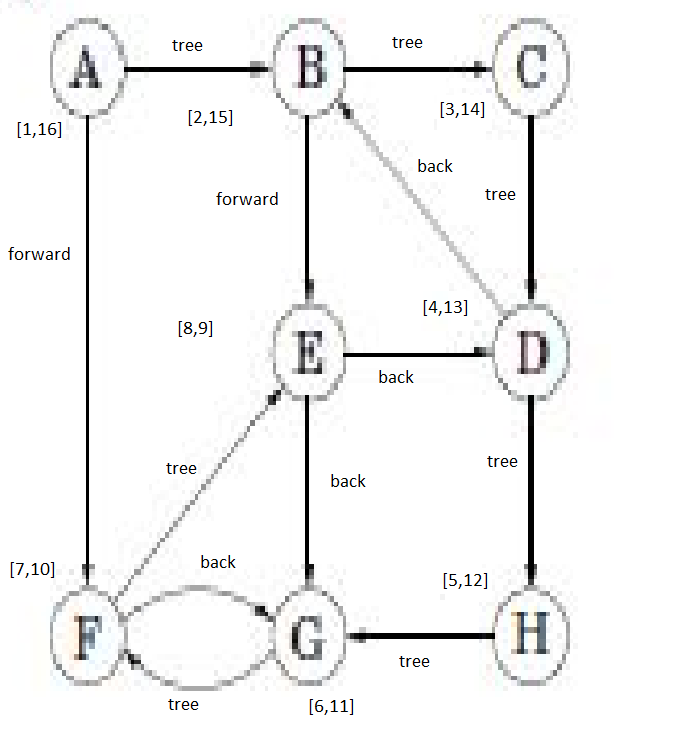
\includegraphics{dfp}

    \clearpage

    \item \begin{enumerate}[(a)]
        \item Let G be the graph where each vertex is represented as ($A_{0}, A_{1}, A_{2}$) where $A_{i}$ is the amount in container i. The container amounts must also always equal to 11,
        since it is our starting amount. An edge between two different vertices ($A_{0}, A_{1}, A_{2}$) and ($B_{0}, B_{1}, B_{2}$) exists if the vertices differ in exactly two coordinates and if one
        of the two differing coordinates is equal to 0.
        \item Given the graph, which is a tree, a depth first search starting from vertex (0, 7, 4) until reaching the desired coordinates would be ideal. Using a depth first search, we find the path
        (0, 7, 4) - (4, 7, 0) - (10, 1, 0) - (6, 1, 4) - (6, 5, 0) - (2, 5, 4) - (2, 7, 2).
    \end{enumerate}
	
\end{enumerate}
\end{document}